\documentclass[conference]{IEEEtran}
\usepackage{graphicx}
\usepackage{booktabs}
\usepackage[backend=biber,style=numeric]{biblatex}
\addbibresource{references.bib}

\title{The Evolution of Super Mario and Nintendo}
\author{
  \IEEEauthorblockN{Your Name}
  \IEEEauthorblockA{Your Affiliation\\
  Your Address\\
  Email: your.email@example.com}
}

\begin{document}

\maketitle

\begin{abstract}
This paper explores the evolution of Super Mario and the impact of Nintendo on the gaming world. It highlights key milestones and innovations that have made Super Mario and Nintendo iconic in the video game industry.
\end{abstract}

\section{Introduction}
Super Mario, the iconic character created by Nintendo, has been a staple in the video game industry for decades. This article explores the evolution of Super Mario and the impact of Nintendo on the gaming world.

\section{The Birth of Super Mario}
Super Mario first appeared in the game "Donkey Kong" in 1981 \cite{ref1}. The character was initially known as "Jumpman" and was created by Shigeru Miyamoto \cite{ref2}. The game was a massive success and paved the way for the creation of the Super Mario Bros. series.

\section{The Rise of Nintendo}
Nintendo, founded in 1889, started as a playing card company \cite{ref3}. It wasn't until the 1970s that Nintendo ventured into the video game industry \cite{ref4}. The release of the Nintendo Entertainment System (NES) in 1985 marked a turning point for the company \cite{ref5}.

\section{Super Mario Games}
The Super Mario Bros. series has seen numerous iterations over the years. Some of the most notable games include "Super Mario Bros." (1985), "Super Mario World" (1990), and "Super Mario Odyssey" (2017) \cite{ref6, ref7, ref8}.

\section{Tables and Figures}

\subsection{Tables}

\begin{table}[h!]
\centering
\begin{tabular}{|c|c|c|}
\hline
Game & Release Year & Platform \\
\hline
Super Mario Bros. & 1985 & NES \\
Super Mario World & 1990 & SNES \\
Super Mario Odyssey & 2017 & Nintendo Switch \\
\hline
\end{tabular}
\caption{Notable Super Mario Games}
\label{table:games}
\end{table}

\begin{table}[h!]
\centering
\begin{tabular}{|c|c|}
\hline
Console & Release Year \\
\hline
NES & 1985 \\
SNES & 1990 \\
Nintendo Switch & 2017 \\
\hline
\end{tabular}
\caption{Nintendo Consoles}
\label{table:consoles}
\end{table}

\subsection{Figures}

\begin{figure}[h!]
\centering
\includegraphics[width=0.5\columnwidth]{super_mario.png}
\caption{Super Mario}
\label{fig:mario}
\end{figure}

\begin{figure}[h!]
\centering
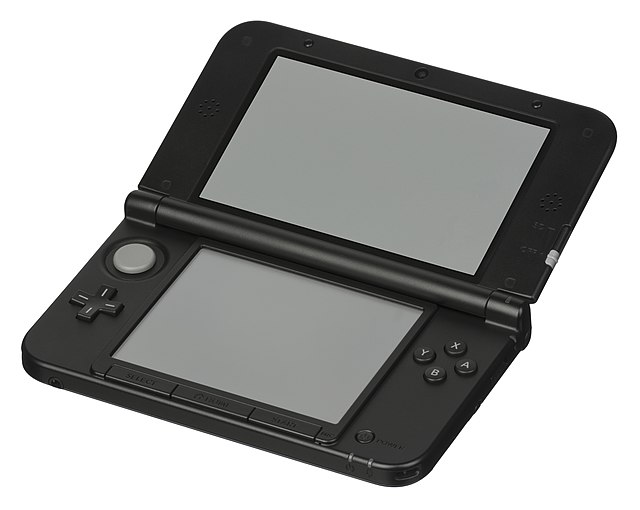
\includegraphics[width=0.5\columnwidth]{nintendo_logo.png}
\caption{Nintendo Logo}
\label{fig:nintendo}
\end{figure}

\section{Conclusion}
Super Mario and Nintendo have left an indelible mark on the video game industry. Their continuous innovation and dedication to quality have made them household names \cite{ref9, ref10}.

\printbibliography

\end{document}

